\scanpage{44}
A) Groupe algébrique \deleted{\unsure{$G$|$E$}}\unsure{[|(}réductif] $G$ sur $\mathbb{Q}$

B) fibre principal à connexion intégrable $\unsure{P|\mathbb P}$ sur $G_S$

% slanted; marginal brace extends alongside C) and D)
\margin{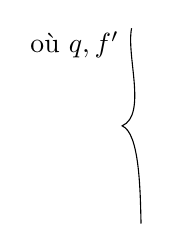
\begin{tikzpicture}[x=1cm,y=1cm,baseline=(current bounding box.north)]
\node[anchor=north east,inner sep=1pt] at (-.09,0) {où $q,f'$};
\draw (.03,0) .. controls (-.04,-.35) and (.23,-1.10) .. (-.09,-1.24)
.. controls (.13,-1.33) and (.14,-2.05) .. (.15,-2.48);
\end{tikzpicture}}
C) Restriction du groupe $G_{\mathbb{C}}^{\mathrm{an}}$ à $G(\mathbb{Q})$ dans $P_{\mathbb{C}}^{\mathrm{an}}$, d'où
\diagram{\begin{tikzcd}[ampersand replacement=\&,column sep=2em]
\text{rev.}\quad\deleted{\unsure{\bar S|\widetilde S}}\quad\widetilde P \arrow[r,hook,"p"] \& P_{\mathbb{C}}^{\mathrm{an}} \arrow[r] \& P
\end{tikzcd}}

D) Application holomorphe
\[
f:\widetilde P\longrightarrow\unsure{\gamma|\mathscr{Y}}_G
\]
satisfaisant $f(xg)=g^{-1}f(x)$ $(x\in\widetilde P,\,g\in G(\mathbb{Q})$ et compatible avec les données B) et $p$ de C).

E) Restriction de $\widetilde P\mathbin{\times}^{G(\mathbb{Q})}G(\mathcal A)$ à $S$, avec compatibilité relativement à $G/G^{\circ}$.

NB La connaissance de A) B) C) et de $f(\xi_0)$, où $\xi_0\in\widetilde P$ est au dessus du point générique de $S$ [\uline{Condition} peut-\uline{être superflue}] \margin{??}doit en principe permettre de réconstituer D) tout entier et E) [lorsqu'on sait \deleted{que} que les données proviennent d'une cat. de motifs $M$].

% slanted; boxed marginal note
\margin{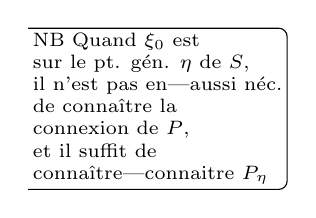
\begin{tikzpicture}[baseline=(current bounding box.north)]
\node[align=left,inner sep=1.5pt,font=\scriptsize] (note) {\uline{NB} Quand $\xi_0$ est\\
sur le pt. gén. $\eta$ de $S$,\\
il n'est pas \deleted{\unsure{en|aussi}} néc.\\
de connaître la\\
connexion de $P$,\\
et il suffit de\\
\unsure{connaître|connaitre} $P_{\eta}$};
\draw[rounded corners=3pt] (note.north west) -- (note.north east) -- (note.south east) -- (note.south west);
\end{tikzpicture}}
\uuline{Formule analytique de prolongement de $f$} ?

\uuline{Relations entre D) et E)} ?? [\unsure{Jugendtraum|Jugend traum} ?]
% archive sheet number: 43
